% Bu dosya hem bağımsız hem de 00_kitap.tex içinden derlenebilir.
\documentclass[00_kitap.tex]{subfiles}

\begin{document}
\BolumKaynakcaBaslat

\setcounter{section}{5}
\section{Kuantum Mekaniğinde İşlemci Yöntemleri}
\label{sec:06_islemci_yontemleri}

Bir önceki bölümde dalga fonksiyonları ile vektörler, özfonksiyon
açılımları ile baz açılımları arasındaki benzerlikleri inceledik.
Bu bölümde aynı yapıyı daha soyut bir gösterimle yeniden kuracağız.
Durumu belirli bir koordinat gösterimine bağlı kalmadan ifade etmek,
birçok işlemi diferansiyel denklem çözmeden yapabilmemizi sağlar.
Burada farklı bir kuantum teorisine değil, aynı teorinin daha genel
bir anlatımına geçiyoruz \cite{book:Gasiorowicz}.

Önce Dirac gösterimini tanıtacak, ardından harmonik salınıcının
enerji spektrumunu merdiven işlemcileriyle elde edeceğiz. Sonra konum
gösterimine dönerek dalga fonksiyonlarını ve Schrödinger denklemini
yeniden bulacağız. Son kısımda zaman gelişiminin Schrödinger,
Heisenberg ve etkileşim resimlerindeki anlatımlarını karşılaştıracağız.

% Kaynak PDF s. 1--13.
\subsection{Kuantum Mekaniğinin Dirac Gösterimiyle Yeniden İfadesi}
\label{sec:06_dirac}

\subsubsection{Ketler, bralar ve iç çarpım}

İncelediğimiz bütün kuantum sistemlerinde \emph{durum} kavramını
kullandık. Örneğin sonsuz kuyunun $n$'inci enerji özdurumu veya
serbest parçacığın bir momentum özdurumu söz konusu olabilir.
Dirac gösteriminde durum vektörleri \emph{ket} olarak adlandırılır ve,
\begin{equation}
 |n\rangle,\qquad |p\rangle,\qquad |\psi\rangle
\end{equation}
ile gösterilir. Ketin içindeki simge bir etikettir. Örneğin
$|n\rangle$ belirli bir bazın elemanını, $|\psi\rangle$ ise genel
bir durumu gösterebilir. Konum veya momentum gibi sürekli spektrum
özketleri, önceki bölümdeki düzlem dalgalar gibi genelleştirilmiş
vektörler olarak kullanılır.

Bir ket iki gözlenebilirin ortak özdurumuysa,
\begin{equation}
 \hat Q|q,r\rangle=q|q,r\rangle,\qquad
 \hat R|q,r\rangle=r|q,r\rangle
\end{equation}
yazabiliriz. $q$ ve $r$ özdeğerleri aynı durumu birlikte etiketler.
Ketlerin doğrusal birleşimi yine bir kettir:
\begin{equation}
 |\Psi\rangle=\alpha|\psi\rangle+\beta|\phi\rangle,
 \qquad \alpha,\beta\in\mathbb C.
 \label{eq:06_superpozisyon}
\end{equation}
Bu vektör sıfırdan farklıysa, fiziksel durum için uygun şekilde
normalize edilebilir.

Her $|\psi\rangle$ ketine karşılık bir eşlenik dual vektör,
\emph{bra}, bulunur:
\begin{equation}
 (|\psi\rangle)^\dagger=\langle\psi|.
\end{equation}
Bu işlem yalnızca karmaşık katsayıların eşleniğini almak değil,
ketten dual uzaydaki braya geçmektir. Örneğin,
\begin{equation}
 (\alpha|\psi\rangle+\beta|\phi\rangle)^\dagger
 =\alpha^*\langle\psi|+\beta^*\langle\phi|.
\end{equation}
Bir bra ile bir ketin iç çarpımı,
\begin{equation}
 \langle\phi|\psi\rangle
\end{equation}
karmaşık bir sayıdır. Konum gösteriminde bunun karşılığı,
\begin{equation}
 \langle\phi|\psi\rangle
 =\int_{-\infty}^{\infty}\phi^*(x)\psi(x)\,dx
 \label{eq:06_ic_carpim}
\end{equation}
olur. Dolayısıyla,
\begin{equation}
 \boxed{\langle\phi|\psi\rangle^*
       =\langle\psi|\phi\rangle}
 \label{eq:06_ic_carpim_eslenik}
\end{equation}
ve,
\begin{align}
 \langle\phi|(\alpha\psi_1+\beta\psi_2)\rangle
 &=\alpha\langle\phi|\psi_1\rangle
   +\beta\langle\phi|\psi_2\rangle,\\
 \langle\alpha\phi_1+\beta\phi_2|\psi\rangle
 &=\alpha^*\langle\phi_1|\psi\rangle
   +\beta^*\langle\phi_2|\psi\rangle
\end{align}
geçerlidir. İç çarpım ket tarafında doğrusal, bra tarafında
eşlenik doğrusaldır. Normalize edilmiş bir durum için,
\begin{equation}
 \langle\psi|\psi\rangle=1
\end{equation}
olur. Ortonormal kesikli bir bazda ise,
\begin{equation}
 \langle m|n\rangle=\delta_{mn}.
 \label{eq:06_baz_ortonormal}
\end{equation}

\subsubsection{İşlemciler ve matris elemanları}

Bir işlemci bir ket üzerinde etki ederek yeni bir ket oluşturur:
\begin{equation}
 \hat Q|\psi\rangle=|\hat Q\psi\rangle.
\end{equation}
Buna soldan $\langle\phi|$ uygulanması,
\begin{equation}
 \langle\phi|\hat Q|\psi\rangle
 =\int\phi^*(x)\hat Q\psi(x)\,dx
 \label{eq:06_matris_elemani}
\end{equation}
matris elemanını verir. Buradaki $\hat Q$, integral içinde aynı
soyut işlemcinin konum gösterimindeki ifadesidir. Matris elemanı
bir sayıdır; genel olarak bir beklenen değer değildir. Normalize
edilmiş aynı durum iki tarafta bulunduğunda,
\begin{equation}
 \langle Q\rangle_\psi=\langle\psi|\hat Q|\psi\rangle
\end{equation}
beklenen değeri elde ederiz.

Hermit eşlenik tanımı bu gösterimde,
\begin{equation}
 \langle\hat Q\phi|\psi\rangle
 =\langle\phi|\hat Q^\dagger|\psi\rangle
\end{equation}
şeklindedir. İç çarpımın eşlenik simetrisiyle,
\begin{equation}
 \boxed{\langle\phi|\hat Q^\dagger|\psi\rangle
       =\langle\psi|\hat Q|\phi\rangle^*}
 \label{eq:06_hermit_eslenik}
\end{equation}
bulunur. Buna karşılık,
\begin{equation}
 (\hat Q|\psi\rangle)^\dagger
 =\langle\psi|\hat Q^\dagger
\end{equation}
olur; eşlenik alınırken çarpanların sırası tersine döner.

Bir uygulama olarak Hermit $\hat Q$ işlemcisinin iki özketini
inceleyelim:
\begin{equation}
 \hat Q|q\rangle=q|q\rangle,\qquad
 \hat Q|r\rangle=r|r\rangle.
\end{equation}
Özdeğerler reel olduğundan,
\begin{align}
 \langle r|\hat Q|q\rangle&=q\langle r|q\rangle,\\
 \langle r|\hat Q|q\rangle
 &=\langle\hat Qr|q\rangle=r\langle r|q\rangle
\end{align}
ve dolayısıyla,
\begin{equation}
 (q-r)\langle r|q\rangle=0
\end{equation}
elde edilir. $q\ne r$ ise özketler diktir. Diklik için bütün
spektrumun dejenere olmaması gerekmez; farklı özdeğerlerin
özketleri her durumda diktir. Aynı özdeğere ait bağımsız ketler
arasından da ortonormal bir baz seçilebilir.

\subsubsection{Açılım ve birim işlemcinin ayrışımı}

Tam ve ortonormal kesikli bir baz için herhangi bir ket,
\begin{equation}
 |\psi\rangle=\sum_n c_n|n\rangle
 \label{eq:06_ket_acilim}
\end{equation}
şeklinde yazılır. $\langle m|$ ile iç çarpım alırsak,
\begin{align}
 \langle m|\psi\rangle
 &=\sum_n c_n\langle m|n\rangle\\
 &=\sum_n c_n\delta_{mn}=c_m
\end{align}
olduğundan,
\begin{equation}
 \boxed{c_n=\langle n|\psi\rangle}
 \label{eq:06_katsayi}
\end{equation}
bulunur. Bu katsayıları açılımda yerlerine koymak,
\begin{equation}
 |\psi\rangle=\sum_n|n\rangle\langle n|\psi\rangle
 =\left(\sum_n|n\rangle\langle n|\right)|\psi\rangle
\end{equation}
verir. Eşitlik bütün uygun ketler için geçerli olduğundan,
\begin{equation}
 \boxed{\sum_n|n\rangle\langle n|=\hat I}
 \label{eq:06_birim}
\end{equation}
\emph{tamlık bağıntısı}na ulaşılır. $\hat I$ birim işlemcidir ve
$\hat I|\psi\rangle=|\psi\rangle$ koşulunu sağlar.

Açılımın Hermit eşleniği ve normu,
\begin{equation}
 \langle\psi|=\sum_n c_n^*\langle n|,
 \qquad\langle\psi|\psi\rangle=\sum_n|c_n|^2=1
 \label{eq:06_norm}
\end{equation}
olur. Böylece önceki bölümde integrallerle yazdığımız sonuçlar
koordinattan bağımsız olarak ifade edilmiş olur.

\subsubsection{Sürekli bazlar ve konum--momentum gösterimleri}

Konumun özketleri,
\begin{equation}
 \hat x|x\rangle=x|x\rangle
\end{equation}
ile tanımlanır. Bunların delta normalizasyonu ve tamlığı,
\begin{equation}
 \langle x|x'\rangle=\delta(x-x'),\qquad
 \boxed{\int_{-\infty}^{\infty}|x\rangle\langle x|\,dx=\hat I}
 \label{eq:06_x_tamlik}
\end{equation}
biçimindedir. Genel ket,
\begin{equation}
 |\psi\rangle=\int|x\rangle\langle x|\psi\rangle\,dx
 =\int\psi(x)|x\rangle\,dx
\end{equation}
olarak açılır. Böylece konum uzayındaki dalga fonksiyonunun,
\begin{equation}
 \boxed{\psi(x)=\langle x|\psi\rangle}
 \label{eq:06_konum_gosterimi}
\end{equation}
olduğunu görürüz. $|\psi\rangle$ soyut durum vektörü, $\psi(x)$
ise onun konum bazındaki bileşenidir; bunlar aynı tür matematiksel
nesneler değildir.

Momentum için benzer şekilde,
\begin{equation}
 \hat p|p\rangle=p|p\rangle,\quad
 \langle p|p'\rangle=\delta(p-p'),\quad
 \int|p\rangle\langle p|\,dp=\hat I
 \label{eq:06_p_tamlik}
\end{equation}
ve,
\begin{equation}
 \boxed{\phi(p)=\langle p|\psi\rangle}
\end{equation}
yazılır. Bu sürekli özketler birim normlu fiziksel dalga paketleri
değildir; delta normalizasyonu dağılımlar anlamında kullanılır.
$|\psi(x)|^2dx$ ve $|\phi(p)|^2dp$ ilgili küçük aralıklarda ölçüm
olasılıklarını verir.

Tamlık bağıntısını iki durum arasına yerleştirerek,
\begin{align}
 \langle\phi|\psi\rangle
 &=\langle\phi|\hat I|\psi\rangle\\
 &=\int\langle\phi|x\rangle\langle x|\psi\rangle\,dx
 =\int\phi^*(x)\psi(x)\,dx
\end{align}
elde ederiz. Aynı yöntemi $\psi(x)$ için momentum bazıyla kullanalım:
\begin{align}
 \psi(x)&=\langle x|\hat I|\psi\rangle\\
 &=\int\langle x|p\rangle\langle p|\psi\rangle\,dp
 =\int\langle x|p\rangle\phi(p)\,dp.
\end{align}
Önceki bölümdeki Fourier açılımıyla karşılaştırıldığında,
\begin{equation}
 \boxed{\langle x|p\rangle
 =\frac{1}{\sqrt{2\pi\hbar}}e^{ipx/\hbar}}
 \label{eq:06_xp_cekirdek}
\end{equation}
olduğu görülür. Bu ifade $|p\rangle$ özketinin konum gösterimidir.
$\langle p|x\rangle=\langle x|p\rangle^*$ olduğundan ters dönüşüm,
\begin{equation}
 \phi(p)=\int\langle p|x\rangle\psi(x)\,dx
 =\frac{1}{\sqrt{2\pi\hbar}}\int e^{-ipx/\hbar}\psi(x)\,dx
\end{equation}
olur. Dolayısıyla Fourier dönüşümü burada iki farklı baz arasındaki
geçiş olarak ortaya çıkar.

\begin{table}[hbtp]
 \centering
 \begin{tabular}{ll}
 \hline
 Soyut ifade & Konum gösterimindeki karşılığı\\
 \hline
 $|\psi\rangle$ durumunun bileşeni & $\psi(x)=\langle x|\psi\rangle$\\
 $|n\rangle$ özketinin bileşeni & $u_n(x)=\langle x|n\rangle$\\
 $\langle\phi|\psi\rangle$ & $\displaystyle\int\phi^*(x)\psi(x)\,dx$\\[5pt]
 $\langle\phi|\hat Q|\psi\rangle$ & $\displaystyle\int\phi^*(x)\hat Q\psi(x)\,dx$\\[5pt]
 $\hat I=\sum_n|n\rangle\langle n|$ & $\displaystyle\sum_n u_n(x)u_n^*(y)=\delta(x-y)$\\[5pt]
 \hline
 \end{tabular}
 \caption{Dirac gösterimi ile konum gösterimi arasındaki temel
 eşlemeler. Son satır tam ve ortonormal kesikli bir baz içindir.}
 \label{tab:06_dirac_esleme}
\end{table}

\subsubsection{İzdüşüm işlemcileri}

Normalize edilmiş bir $|n\rangle$ için,
\begin{equation}
 \hat P_n\equiv|n\rangle\langle n|
 \label{eq:06_projektor}
\end{equation}
\emph{izdüşüm işlemcisi}ni tanımlayalım. Bu dış çarpım bir sayı
değil, ketlere etki eden bir işlemcidir:
\begin{equation}
 \hat P_n|\psi\rangle
 =|n\rangle\langle n|\psi\rangle=c_n|n\rangle.
 \label{eq:06_projektor_etki}
\end{equation}
Buna karşılık ölçüm olasılığı,
\begin{equation}
 \boxed{P(n)=|c_n|^2
 =\langle\psi|n\rangle\langle n|\psi\rangle
 =\langle\psi|\hat P_n|\psi\rangle}
 \label{eq:06_olasilik}
\end{equation}
bir sayıdır. $|c_n|^2$ ile $|n\rangle\langle n|$ birbirine eşit
değildir; ikincisinin uygun durumdaki beklenen değeri birinciyi verir.

Ortonormal ketler için,
\begin{align}
 \hat P_m\hat P_n
 &=|m\rangle\langle m|n\rangle\langle n|
 =\delta_{mn}|n\rangle\langle n|
 =\delta_{mn}\hat P_n,\\
 \hat P_n^\dagger&=\hat P_n,\qquad
 \hat P_n^2=\hat P_n,\qquad
 \sum_n\hat P_n=\hat I
 \label{eq:06_projektor_ozellik}
\end{align}
olur. Özellikle $\hat P_n^2=\hat P_n$ özelliği, bir kere seçilmiş
bileşene aynı izdüşümün tekrar uygulanmasının onu değiştirmediğini
gösterir. İdeal bir projektif ölçümde $n$ sonucu elde edilirse,
$P(n)>0$ için normalize edilmiş ölçüm sonrası ket,
\begin{equation}
 |\psi_{\rm son}\rangle
 =\frac{\hat P_n|\psi\rangle}{\sqrt{P(n)}}
\end{equation}
olur. $c_n$ genel olarak karmaşık olduğundan bu ket $|n\rangle$'ye
bir genel faz dışında eşittir. Dejenerelik varsa bir özdeğerin
projektörü, o özuzaydaki ortonormal baz ketlerinin projektörlerinin
toplamıdır.

\begin{figure}[hbtp]
 \centering
 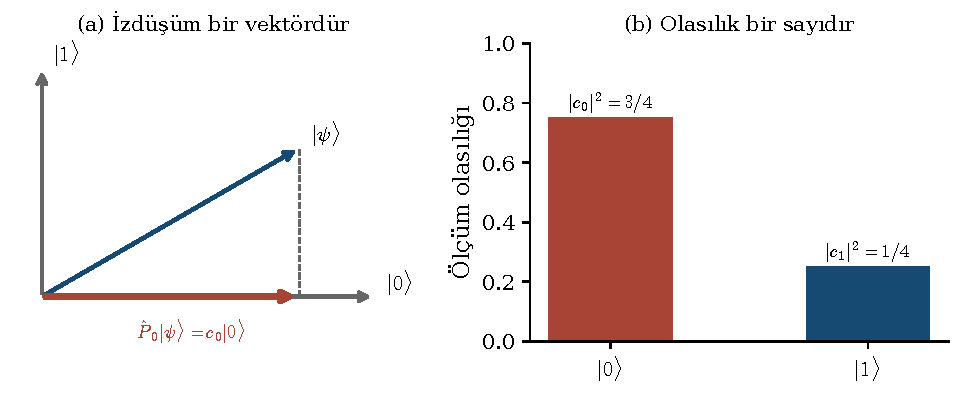
\includegraphics[width=\linewidth]{figurler/06_izdusum.pdf}
 \caption[İzdüşüm ile olasılığın ayrılması]{İki reel katsayılı
 $|\psi\rangle=(\sqrt3/2)|0\rangle+(1/2)|1\rangle$ örneğinde
 izdüşüm ve olasılık. Solda izdüşümün ürettiği vektör, sağda
 projektörün beklenen değeri olan ölçüm olasılıkları gösterilir.}
 \label{fig:06_izdusum}
\end{figure}

\subsubsection{Beklenen değer ve işlemcinin spektral açılımı}

Enerji özketleri $\hat H|n\rangle=E_n|n\rangle$ koşulunu sağlasın.
Tamlık kullanıldığında,
\begin{align}
 \langle H\rangle
 &=\langle\psi|\hat H\left(\sum_n|n\rangle\langle n|\right)
                  |\psi\rangle\\
 &=\sum_n E_n\langle\psi|n\rangle\langle n|\psi\rangle
 =\boxed{\sum_n E_n|c_n|^2}
 \label{eq:06_enerji_ortalama}
\end{align}
elde edilir. Aynı hesap yalnızca beklenen değeri değil işlemcinin
kendisini de özketleri cinsinden yazmamızı sağlar:
\begin{equation}
 \boxed{\hat H=\sum_n E_n|n\rangle\langle n|
              =\sum_n E_n\hat P_n.}
 \label{eq:06_spektral}
\end{equation}
Bu, Hamiltonyenin \emph{spektral ayrışımı}dır. Kesikli ve sürekli
bileşenler birlikte varsa gerekli integraller de eklenir. Aynı
özdeğere ait birden fazla ket bulunuyorsa bunlar aynı özuzayın
projektörü altında toplanabilir.

% Kaynak PDF s. 14--24.
\subsection{Harmonik Salınıcının Enerji Spektrumu}
\label{sec:06_harmonik}

Bir boyutlu harmonik salınıcının Hamiltonyeni,
\begin{equation}
 \hat H=\frac{\hat p^2}{2m}+\frac12m\omega^2\hat x^2
 \label{eq:06_ho_hamiltonyen}
\end{equation}
şeklindedir. $\hat x$ ve $\hat p$ Hermit işlemcilerdir; uygun ortak
tanım kümesinde temel komütasyon bağıntıları,
\begin{equation}
 [\hat x,\hat p]=i\hbar\hat I,\qquad
 [\hat p,\hat x]=-i\hbar\hat I
\end{equation}
olur. Bu bölümde aynı bağıntıları kullanarak enerji spektrumunu
diferansiyel denklem çözmeden elde edeceğiz.

\subsubsection{Hamiltonyenin çarpanlara ayrılması}

Boyutsuz iki işlemci tanımlayalım:
\begin{align}
 \hat A&=\sqrt{\frac{m\omega}{2\hbar}}\,\hat x
       +\frac{i}{\sqrt{2m\omega\hbar}}\,\hat p,\\
 \hat A^\dagger&=\sqrt{\frac{m\omega}{2\hbar}}\,\hat x
       -\frac{i}{\sqrt{2m\omega\hbar}}\,\hat p.
 \label{eq:06_merdiven_tanim}
\end{align}
Bunlar birbirinin Hermit eşleniğidir; tek tek Hermit değildir.
Burada $\hat A$ ve $\hat A^\dagger$ gösterimini kullanıyoruz;
kitaplarda sıklıkla $\hat a$ ve $\hat a^\dagger$ de kullanılır.

Çarpımı açıkça hesaplarsak,
\begin{align}
 \hat A^\dagger\hat A
 &=\frac{m\omega}{2\hbar}\hat x^2
   +\frac{1}{2m\omega\hbar}\hat p^2
   +\frac{i}{2\hbar}(\hat x\hat p-\hat p\hat x)\\
 &=\frac{\hat H}{\hbar\omega}-\frac12\hat I
 \label{eq:06_adaga_acilim}
\end{align}
olur. Dolayısıyla,
\begin{equation}
 \boxed{\hat H=\hbar\omega
                  \left(\hat A^\dagger\hat A+\frac12\hat I\right)}
 \label{eq:06_ho_carpan}
\end{equation}
biçimi elde edilir. Buradaki $\hbar\omega/2$ terimi işlemcilerin
komüte etmemesinden doğar; klasik $x$ ve $p$ sayılarıyla aynı
çarpanlara ayırma yapılsaydı bu katkı ortaya çıkmazdı.

\subsubsection{Merdiven işlemcilerinin komütatörleri}

Hesabı kısaltmak için geçici olarak,
\begin{equation}
 \hat X=\sqrt{\frac{m\omega}{2\hbar}}\hat x,
 \qquad \hat P=\frac{\hat p}{\sqrt{2m\omega\hbar}}
\end{equation}
yazalım. Buradaki $\hat P$ boyutsuz momentumdur; izdüşüm
işlemcisi $\hat P_n$ ile karıştırılmamalıdır. Böylece
$\hat A=\hat X+i\hat P$, $\hat A^\dagger=\hat X-i\hat P$
ve $[\hat X,\hat P]=i\hat I/2$ olur. Adım adım,
\begin{align}
 [\hat A,\hat A^\dagger]
 &=[\hat X+i\hat P,\hat X-i\hat P]\\
 &=-i[\hat X,\hat P]+i[\hat P,\hat X]\\
 &=-2i[\hat X,\hat P]=\hat I
\end{align}
elde edilir. Yani,
\begin{equation}
 \boxed{[\hat A,\hat A^\dagger]=\hat I,\qquad
 \hat A\hat A^\dagger=\hat A^\dagger\hat A+\hat I.}
 \label{eq:06_aa_komutator}
\end{equation}
Komütatörün çarpım kuralını kullanarak,
\begin{align}
 [\hat H,\hat A]
 &=\hbar\omega[\hat A^\dagger\hat A,\hat A]\\
 &=\hbar\omega\bigl(\hat A^\dagger[\hat A,\hat A]
             +[\hat A^\dagger,\hat A]\hat A\bigr)
 =-\hbar\omega\hat A,\\
 [\hat H,\hat A^\dagger]
 &=\hbar\omega\hat A^\dagger[\hat A,\hat A^\dagger]
 =+\hbar\omega\hat A^\dagger
 \label{eq:06_h_merdiven}
\end{align}
bulunur. Bu bağıntılar merdiven yapısının temelidir.

\subsubsection{Enerjiyi azaltma ve artırma}

$|E\rangle$ normalize edilebilir bir enerji özketi olsun:
\begin{equation}
 \hat H|E\rangle=E|E\rangle.
\end{equation}
Denk.~\eqref{eq:06_h_merdiven}'deki ilk bağıntı bu ket üzerinde,
\begin{align}
 (\hat H\hat A-\hat A\hat H)|E\rangle
 &=-\hbar\omega\hat A|E\rangle,\\
 \hat H(\hat A|E\rangle)
 &=(E-\hbar\omega)(\hat A|E\rangle)
 \label{eq:06_alcaltma_enerji}
\end{align}
verir. Dolayısıyla $\hat A|E\rangle$ sıfır vektörü değilse,
enerjisi $\hbar\omega$ daha düşük bir özkettir. Benzer şekilde,
\begin{equation}
 \hat H(\hat A^\dagger|E\rangle)
 =(E+\hbar\omega)(\hat A^\dagger|E\rangle)
 \label{eq:06_yukseltme_enerji}
\end{equation}
olur. Bu nedenle $\hat A$ \emph{alçaltma}, $\hat A^\dagger$
\emph{yükseltme} işlemcisi olarak adlandırılır. Her ikisine birlikte
\emph{merdiven işlemcileri} denir.

Buradaki enerji basamakları bir cebirsel ilişkidir. $\hat A$ veya
$\hat A^\dagger$ uygulamak tek başına sistemin kendiliğinden fiziksel
bir geçiş yapacağını söylemez; gerçek bir geçişi oluşturacak
etkileşim ayrıca belirtilmelidir.

\begin{figure}[hbtp]
 \centering
 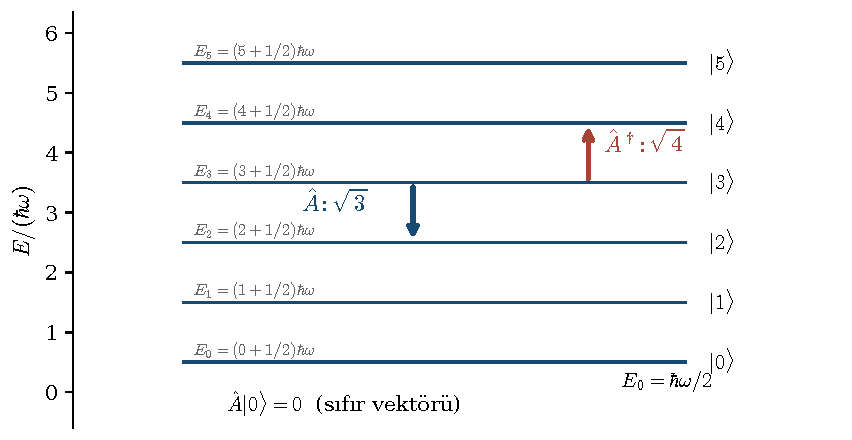
\includegraphics[width=.94\linewidth]{figurler/06_merdiven.pdf}
 \caption[Harmonik salınıcının merdiven yapısı]{Harmonik salınıcının
 eşit aralıklı enerji merdiveni. Oklar örnek olarak $|3\rangle$
 durumuna alçaltma ve yükseltme uygulanmasını gösterir; yanlarındaki
 karekökler oluşan normalize edilmemiş ketin katsayılarıdır.
 $\hat A|0\rangle=0$ ifadesi daha aşağıda bir enerji durumu değil,
 sıfır vektörünü verir.}
 \label{fig:06_merdiven}
\end{figure}

\subsubsection{Alt sınır, taban durumu ve sıfır nokta enerjisi}

Hamiltonyenin iki terimi de pozitif yarı tanımlıdır:
\begin{equation}
 \langle\psi|\hat p^2|\psi\rangle
 =\|\hat p|\psi\rangle\|^2\ge0,\qquad
 \langle\psi|\hat x^2|\psi\rangle
 =\|\hat x|\psi\rangle\|^2\ge0.
\end{equation}
Böylece enerji sınırsız biçimde aşağı indirilemez.
Denk.~\eqref{eq:06_ho_carpan} daha güçlü bir alt sınır verir:
\begin{equation}
 \langle H\rangle
 =\hbar\omega\left(\|\hat A|\psi\rangle\|^2+\frac12\right)
 \ge\frac12\hbar\omega
 \label{eq:06_enerji_alt_sinir}
\end{equation}
($\langle\psi|\psi\rangle=1$). Bir enerji özdurumuna $\hat A$
art arda uygulanırken her adımda enerji $\hbar\omega$ azalır.
Sıfırdan farklı ketler sonsuza kadar üretilemez; aksi halde enerji
bu alt sınırın altına inerdi. Zincir bir taban ketinde sonlanmalıdır:
\begin{equation}
 \boxed{\hat A|0\rangle=0.}
 \label{eq:06_vakum}
\end{equation}
Burada $|0\rangle$ sıfır vektörü değildir; normalize edilmiş
\emph{taban durumu} veya \emph{vakum} ketidir. $0$ yalnızca en
küçük basamağın etiketidir. Hamiltonyen uygulandığında,
\begin{equation}
 \hat H|0\rangle
 =\hbar\omega\left(\hat A^\dagger\hat A+\frac12\hat I\right)
 |0\rangle=\frac12\hbar\omega|0\rangle
\end{equation}
olduğundan,
\begin{equation}
 \boxed{E_0=\frac12\hbar\omega}
\end{equation}
\emph{sıfır nokta enerjisi} bulunur.

Bu sonucu belirsizlik ilkesiyle de ilişkilendirebiliriz. Genel bir
normalize edilmiş durumda,
\begin{equation}
 \langle H\rangle
 =\frac{\langle p\rangle^2+(\Delta p)^2}{2m}
 +\frac12m\omega^2\bigl[\langle x\rangle^2+(\Delta x)^2\bigr].
\end{equation}
Ortalama konum ve momentum sıfırken bile dalgalanma terimleri kalır.
Aritmetik--geometrik ortalama eşitsizliği ve belirsizlik ilkesiyle,
\begin{equation}
 \frac{(\Delta p)^2}{2m}+\frac12m\omega^2(\Delta x)^2
 \ge\omega\Delta x\Delta p\ge\frac12\hbar\omega
\end{equation}
olur. Dolayısıyla taban durumu, $x=0$ ve $p=0$ değerlerinin ikisinin
de kesin olduğu klasik hareketsiz durum değildir.

Taban durumuna $n$ defa yükseltme uygulandığında,
\begin{equation}
 \boxed{E_n=\hbar\omega\left(n+\frac12\right),
 \qquad n=0,1,2,\ldots}
 \label{eq:06_spektrum}
\end{equation}
elde edilir. Böylece daha önce seri çözümüyle bulduğumuz enerji
spektrumuna yalnızca işlemci cebiriyle ulaştık.

\subsubsection{Üretilen ketlerin normalizasyonu}

Şimdi $(\hat A^\dagger)^n|0\rangle$ ketlerinin normunu bulalım.
Önce $\hat A\hat A^\dagger=\hat I+\hat A^\dagger\hat A$
bağıntısını art arda kullanarak,
\begin{align}
 \hat A(\hat A^\dagger)^n
 &=(\hat I+\hat A^\dagger\hat A)(\hat A^\dagger)^{n-1}\\
 &=(\hat A^\dagger)^{n-1}
   +\hat A^\dagger\hat A(\hat A^\dagger)^{n-1}\\
 &=2(\hat A^\dagger)^{n-1}
   +(\hat A^\dagger)^2\hat A(\hat A^\dagger)^{n-2}\\
 &=n(\hat A^\dagger)^{n-1}+(\hat A^\dagger)^n\hat A
 \label{eq:06_normal_siralama}
\end{align}
elde edilir. Son eşitlik $n\ge1$ için geçerlidir. Taban ketine
uygulandığında son terim sıfır olur:
\begin{equation}
 \hat A(\hat A^\dagger)^n|0\rangle
 =n(\hat A^\dagger)^{n-1}|0\rangle.
\end{equation}
Bir kez daha alçaltmak,
\begin{equation}
 \hat A^2(\hat A^\dagger)^n|0\rangle
 =n(n-1)(\hat A^\dagger)^{n-2}|0\rangle
\end{equation}
verir. Genel sonuç,
\begin{equation}
 \hat A^r(\hat A^\dagger)^n|0\rangle
 =\begin{cases}
 \displaystyle\frac{n!}{(n-r)!}
       (\hat A^\dagger)^{n-r}|0\rangle,&0\le r\le n,\\[5pt]
 0,&r>n
 \end{cases}
 \label{eq:06_tekrarli_alcaltma}
\end{equation}
şeklindedir. Kuvvet indisini $r$ seçerek kütle $m$ ile karışmasını
önlüyoruz. Özellikle,
\begin{equation}
 \hat A^n(\hat A^\dagger)^n|0\rangle=n!|0\rangle
\end{equation}
olduğundan, $\langle0|0\rangle=1$ için,
\begin{equation}
 \|(\hat A^\dagger)^n|0\rangle\|^2
 =\langle0|\hat A^n(\hat A^\dagger)^n|0\rangle=n!
\end{equation}
bulunur. Normalize edilmiş enerji özketleri böylece,
\begin{equation}
 \boxed{|n\rangle=\frac{(\hat A^\dagger)^n}{\sqrt{n!}}|0\rangle,
 \qquad\langle n|=\langle0|\frac{\hat A^n}{\sqrt{n!}}}
 \label{eq:06_fock_ket}
\end{equation}
ile tanımlanır.

Farklı enerji özdeğerlerine sahip olduklarından bu ketler diktir.
Bunu vakum matris elemanı üzerinden de yazabiliriz:
\begin{equation}
 \boxed{\langle0|\hat A^r(\hat A^\dagger)^n|0\rangle
        =n!\delta_{rn}.}
 \label{eq:06_vakum_carpim}
\end{equation}
$r<n$ için geriye daha yüksek enerjili bir ket kalır ve
$\langle0|$ ile iç çarpımı sıfırdır. $r>n$ için alçaltma taban
ketini yok eder. $r=n$ için sonuç $n!$'dir. Dolayısıyla,
\begin{equation}
 \langle r|n\rangle
 =\frac{1}{\sqrt{r!n!}}
 \langle0|\hat A^r(\hat A^\dagger)^n|0\rangle=\delta_{rn}
\end{equation}
ortonormalliği açıkça sağlanır.

\subsubsection{Normalize edilmiş ketlere etki ve sayı işlemcisi}

Denk.~\eqref{eq:06_fock_ket}'ten,
\begin{align}
 |n+1\rangle
 &=\frac{(\hat A^\dagger)^{n+1}}{\sqrt{(n+1)!}}|0\rangle
 =\frac{\hat A^\dagger}{\sqrt{n+1}}|n\rangle,\\
 \hat A|n\rangle
 &=\frac{n}{\sqrt{n!}}(\hat A^\dagger)^{n-1}|0\rangle
 =\sqrt n\,|n-1\rangle
\end{align}
olduğundan,
\begin{equation}
 \boxed{\hat A^\dagger|n\rangle=\sqrt{n+1}|n+1\rangle,
 \qquad \hat A|n\rangle=\sqrt n\,|n-1\rangle.}
 \label{eq:06_merdiven_etki}
\end{equation}
İkinci ifade $n\ge1$ içindir; $n=0$ için sonuç doğrudan sıfırdır.
$|-1\rangle$ diye bir enerji özketi tanımlamıyoruz.

$\hat N=\hat A^\dagger\hat A$ \emph{sayı işlemcisi} olarak
adlandırılır ve,
\begin{equation}
 \hat N|n\rangle=n|n\rangle,\qquad
 \hat A\hat A^\dagger|n\rangle=(n+1)|n\rangle
\end{equation}
koşullarını sağlar. Bu nedenle,
\begin{equation}
 \langle n|\hat A^\dagger\hat A|n\rangle=n,
 \quad\langle n|\hat A\hat A^\dagger|n\rangle=n+1,
 \quad\langle n|\hat H|n\rangle=E_n.
\end{equation}
Hamiltonyenin eşdeğer biçimleri,
\begin{equation}
 \hat H=\hbar\omega\left(\hat N+\frac12\hat I\right)
 =\hbar\omega\left(\hat A\hat A^\dagger-\frac12\hat I\right)
 =\frac{\hbar\omega}{2}
    (\hat A^\dagger\hat A+\hat A\hat A^\dagger)
\end{equation}
olarak da yazılır. Konum ve momentum işlemcileri ise tanım
bağıntıları ters çevrilerek,
\begin{equation}
 \hat x=\sqrt{\frac{\hbar}{2m\omega}}(\hat A+\hat A^\dagger),
 \qquad
 \hat p=-i\sqrt{\frac{m\hbar\omega}{2}}(\hat A-\hat A^\dagger)
 \label{eq:06_xp_merdiven}
\end{equation}
şeklinde elde edilir.

% Kaynak PDF s. 25--28.
\subsection{Bra--Ket Gösterimiyle Schrödinger Denklemi}
\label{sec:06_bra_ket_sch}

Soyut işlemci çözümünden yeniden konum gösterimine dönelim.
Taban durumunun $\hat A|0\rangle=0$ koşulunu soldan
$\langle x|$ ile çarparsak,
\begin{equation}
 \langle x|\hat A|0\rangle=0
 \label{eq:06_vakum_konum}
\end{equation}
elde ederiz. Amacımız bu koşuldan $u_0(x)=\langle x|0\rangle$
fonksiyonunu bulmaktır.

\subsubsection{Konum gösteriminde momentumun türev olması}

Önce $\langle x|\hat p|\psi\rangle$ ifadesini hesaplayalım.
Momentum bazının tamlığını yerleştirirsek,
\begin{align}
 \langle x|\hat p|\psi\rangle
 &=\int\langle x|\hat p|p\rangle\langle p|\psi\rangle\,dp\\
 &=\int p\langle x|p\rangle\langle p|\psi\rangle\,dp\\
 &=\frac{1}{\sqrt{2\pi\hbar}}
      \int p\,e^{ipx/\hbar}\phi(p)\,dp
\end{align}
olur. $p e^{ipx/\hbar}=(\hbar/i)\partial_xe^{ipx/\hbar}$
olduğundan ve türev ile integralin yer değiştirebildiği uygun
durumlarda,
\begin{align}
 \langle x|\hat p|\psi\rangle
 &=\frac{\hbar}{i}\frac{\partial}{\partial x}
      \int\langle x|p\rangle\langle p|\psi\rangle\,dp\\
 &=\frac{\hbar}{i}\frac{\partial}{\partial x}
      \langle x|\hat I|\psi\rangle
 =-i\hbar\frac{\partial\psi(x)}{\partial x}
 \label{eq:06_p_turev}
\end{align}
bulunur. Benzer biçimde,
\begin{equation}
 \langle x|\hat x|\psi\rangle=x\psi(x)
\end{equation}
olur. Böylece konum ve momentumun alışılmış çarpma ve türev
ifadeleri, soyut ketler arasındaki baz dönüşümünden elde edilmiştir.

\subsubsection{Taban durum dalga fonksiyonu}

Denk.~\eqref{eq:06_merdiven_tanim}'i
Denk.~\eqref{eq:06_vakum_konum}'da kullanarak,
\begin{equation}
 \sqrt{\frac{m\omega}{2\hbar}}\langle x|\hat x|0\rangle
 +\frac{i}{\sqrt{2m\omega\hbar}}\langle x|\hat p|0\rangle=0
\end{equation}
yazarız. Az önceki sonuçları yerlerine koyup
$\sqrt{2m\omega\hbar}$ ile çarparsak,
\begin{equation}
 m\omega x\langle x|0\rangle
 +\hbar\frac{d}{dx}\langle x|0\rangle=0
\end{equation}
bulunur. $u_0(x)=\langle x|0\rangle$ tanımıyla,
\begin{equation}
 \left(m\omega x+\hbar\frac{d}{dx}\right)u_0(x)=0
\end{equation}
birinci mertebeden diferansiyel denklemine ulaşılır. Çözümü,
\begin{equation}
 u_0(x)=C\exp\left(-\frac{m\omega x^2}{2\hbar}\right)
\end{equation}
şeklindedir. Normalizasyon,
\begin{equation}
 1=|C|^2\int_{-\infty}^{\infty}e^{-m\omega x^2/\hbar}\,dx
 =|C|^2\sqrt{\frac{\pi\hbar}{m\omega}}
\end{equation}
verir. Genel fazı sıfır seçerek,
\begin{equation}
 \boxed{u_0(x)=\left(\frac{m\omega}{\pi\hbar}\right)^{1/4}
              \exp\left(-\frac{m\omega x^2}{2\hbar}\right)}
 \label{eq:06_taban_df}
\end{equation}
elde ederiz. Yani ikinci mertebeden Schrödinger denklemini doğrudan
çözmeden taban durumunu bulduk.

\subsubsection{Üst durumların üretilmesi}

Uzunluk ölçeği $\ell=\sqrt{\hbar/(m\omega)}$ kullanılırsa
merdiven işlemcilerinin konum gösterimi,
\begin{equation}
 \hat A=\frac{1}{\sqrt2}
    \left(\frac{x}{\ell}+\ell\frac{d}{dx}\right),\qquad
 \hat A^\dagger=\frac{1}{\sqrt2}
    \left(\frac{x}{\ell}-\ell\frac{d}{dx}\right)
 \label{eq:06_merdiven_turev}
\end{equation}
olur. Soyut ket bağıntısı,
\begin{equation}
 |n\rangle=\frac{(\hat A^\dagger)^n}{\sqrt{n!}}|0\rangle
\end{equation}
konum bazında,
\begin{equation}
 \boxed{u_n(x)=\frac{1}{\sqrt{n!}}
 \left[\frac{1}{\sqrt2}
       \left(\frac{x}{\ell}-\ell\frac{d}{dx}\right)\right]^n u_0(x)}
 \label{eq:06_ust_df}
\end{equation}
şeklindedir. Köşeli parantezdeki işlemci bütünüyle $n$ defa
uygulanır; $x$ ile türev komüte etmediği için bu kuvvet sıradan bir
sayısal çarpım gibi açılamaz. İlk iki örnek,
\begin{align}
 u_1(x)&=\sqrt2\frac{x}{\ell}u_0(x),\\
 u_2(x)&=\frac{1}{\sqrt2}
           \left(2\frac{x^2}{\ell^2}-1\right)u_0(x)
\end{align}
olur. Genel sonuç,
\begin{equation}
 u_n(x)=\frac{1}{\pi^{1/4}\sqrt{2^n n!\,\ell}}
        H_n\left(\frac{x}{\ell}\right)e^{-x^2/(2\ell^2)}
\end{equation}
olarak yazılır. Böylece önceki bölümdeki Hermite polinomlu
özfonksiyonlara aynı işlemci yöntemiyle ulaşılmış olur.

\subsubsection{Genel potansiyel için Schrödinger denklemi}

Harmonik salınıcı yerine genel bir yerel skaler potansiyel alalım:
\begin{equation}
 \hat H=\frac{\hat p^2}{2m}+V(\hat x),\qquad
 \hat H|E\rangle=E|E\rangle.
\end{equation}
$u_E(x)=\langle x|E\rangle$ ve
$\langle x|V(\hat x)|E\rangle=V(x)u_E(x)$ olduğuna göre,
\begin{align}
 \langle x|\hat H|E\rangle
 &=-\frac{\hbar^2}{2m}\frac{d^2u_E(x)}{dx^2}
   +V(x)u_E(x)\\
 &=E u_E(x)
\end{align}
elde edilir. Yani,
\begin{equation}
 \boxed{-\frac{\hbar^2}{2m}u_E''(x)+V(x)u_E(x)=E u_E(x)}
\end{equation}
zamandan bağımsız Schrödinger denklemi, soyut enerji özdeğer
denkleminin konum gösterimidir. Aynı şekilde,
\begin{equation}
 i\hbar\frac{d}{dt}|\psi(t)\rangle=\hat H|\psi(t)\rangle
\end{equation}
üzerine $\langle x|$ uygulanması da zamana bağlı Schrödinger
denklemini verir. Böylece soyut işlemci yaklaşımı ile dalga
mekaniğinin aynı fiziksel içeriği taşıdığı açıkça görülür.

% Kaynak PDF s. 29--38.
\subsection{İşlemci ve Dalga Fonksiyonlarının Zamanla Değişimi}
\label{sec:06_zaman}

Bir sistemin zamanla gelişimini Schrödinger, Heisenberg ve
etkileşim (Dirac) resimleriyle tanımlayabiliriz. Bu anlatımlarda
zaman bağımlılığı durum vektörleri ile işlemciler arasında farklı
şekillerde paylaştırılır. Ölçüm olasılıkları ve beklenen değerler
aynıdır.

\subsubsection{Zaman gelişim işlemcisi ve üniterlik}

Schrödinger resmindeki durumun hareket denklemi,
\begin{equation}
 i\hbar\frac{d}{dt}|\psi_S(t)\rangle
 =\hat H_S(t)|\psi_S(t)\rangle
 \label{eq:06_sch_ket}
\end{equation}
olsun. Başlangıç anı $t_0$'dan $t$ anına taşıyan zaman gelişim
işlemcisini,
\begin{equation}
 |\psi_S(t)\rangle=\hat U(t,t_0)|\psi_S(t_0)\rangle
 \label{eq:06_evrim}
\end{equation}
ile tanımlarız. Bu işlemci,
\begin{equation}
 i\hbar\frac{\partial\hat U(t,t_0)}{\partial t}
 =\hat H_S(t)\hat U(t,t_0),\qquad
 \hat U(t_0,t_0)=\hat I
 \label{eq:06_u_denkl}
\end{equation}
koşullarını sağlar. Hamiltonyen zamandan bağımsızsa çözüm,
\begin{equation}
 \boxed{\hat U(t,t_0)=
 \exp\left[-\frac{i}{\hbar}\hat H_S(t-t_0)\right]}
 \label{eq:06_u_ustel}
\end{equation}
olur. Zamana bağlı Hamiltonyen için bu basit üstel genel olarak
kullanılamaz: farklı zamanlardaki Hamiltonyenler komüte etmiyorsa
zaman sıralaması gerekir. Bu durumda da
Denk.~\eqref{eq:06_u_denkl} geçerlidir.

Kendine eşlenik Hamiltonyen için gelişim üniterdir:
\begin{equation}
 \boxed{\hat U^\dagger\hat U=\hat U\hat U^\dagger=\hat I,
        \qquad \hat U^{-1}=\hat U^\dagger.}
 \label{eq:06_uniter}
\end{equation}
Zamandan bağımsız durumda bunu doğrudan gösterebiliriz:
\begin{equation}
 \hat U^\dagger\hat U
 =e^{+i\hat H_S(t-t_0)/\hbar}
  e^{-i\hat H_S(t-t_0)/\hbar}=\hat I.
\end{equation}
Burada iki üstel aynı işlemcinin fonksiyonları olduğu için komüte
eder. Genel zamana bağlı durumda ise,
\begin{equation}
 \frac{d}{dt}(\hat U^\dagger\hat U)
 =\frac{i}{\hbar}\hat U^\dagger\hat H_S\hat U
  -\frac{i}{\hbar}\hat U^\dagger\hat H_S\hat U=0
\end{equation}
ve başlangıç koşulu kullanılır. Üniterlik normu ve iç çarpımları
korur:
\begin{equation}
 \langle\phi(t)|\psi(t)\rangle
 =\langle\phi(t_0)|\hat U^\dagger\hat U|\psi(t_0)\rangle
 =\langle\phi(t_0)|\psi(t_0)\rangle.
\end{equation}
Ayrıca gelişim işlemcileri,
\begin{equation}
 \hat U(t_2,t_1)\hat U(t_1,t_0)=\hat U(t_2,t_0),\qquad
 \hat U(t_0,t)=\hat U(t,t_0)^\dagger
\end{equation}
bileşim ve tersine gelişim bağıntılarını sağlar.

Hamiltonyen zamandan bağımsız ve kesikli bir enerji bazına sahipse,
\begin{align}
 |\psi_S(t_0)\rangle&=\sum_n c_n|n\rangle,\\
 |\psi_S(t)\rangle
 &=\sum_n c_n e^{-iE_n(t-t_0)/\hbar}|n\rangle
 \label{eq:06_faz_evrimi}
\end{align}
olur. Aynı ifadeyi $\hat U$'nun spektral açılımıyla,
\begin{equation}
 \hat U(t,t_0)=\sum_n e^{-iE_n(t-t_0)/\hbar}|n\rangle\langle n|
\end{equation}
yazabiliriz.

\subsubsection{Genel bir üniter gösterim değişimi}

Zaman gelişimini farklı bir resimde anlatmak için üniter bir
$\hat W(t)$ seçelim; $\hat W(t_0)=\hat I$ olsun. Yeni durum vektörü
ve gözlenebilir işlemcisi,
\begin{equation}
 |\psi_T(t)\rangle=\hat W^\dagger(t)|\psi_S(t)\rangle,
 \qquad
 \hat Q_T(t)=\hat W^\dagger(t)\hat Q_S(t)\hat W(t)
 \label{eq:06_genel_donusum}
\end{equation}
ile tanımlanır. Burada $\hat W$ mutlaka tam fiziksel gelişim
$\hat U$ olmak zorunda değildir; farklı seçimler farklı resimleri
verir. Beklenen değer,
\begin{align}
 \langle\psi_T|\hat Q_T|\psi_T\rangle
 &=\langle\psi_S|\hat W\hat W^\dagger
          \hat Q_S\hat W\hat W^\dagger|\psi_S\rangle\\
 &=\boxed{\langle\psi_S|\hat Q_S|\psi_S\rangle}
 \label{eq:06_beklenen_degismez}
\end{align}
olduğundan dönüşüm ölçülebilir sonucu değiştirmez. Projektörler
de aynı biçimde dönüştüğü için bütün ölçüm olasılıkları korunur.

Yeni durumun denklemini türetelim. $|\psi_S\rangle=\hat W|\psi_T\rangle$
ifadesini Schrödinger denklemine koyarsak,
\begin{equation}
 \hat H_S\hat W|\psi_T\rangle
 =i\hbar\dot{\hat W}|\psi_T\rangle
  +i\hbar\hat W\frac{d}{dt}|\psi_T\rangle
\end{equation}
olur. Soldan $\hat W^\dagger$ ile çarparak,
\begin{equation}
 i\hbar\frac{d}{dt}|\psi_T\rangle=\hat K_T|\psi_T\rangle,
 \qquad
 \boxed{\hat K_T=\hat W^\dagger\hat H_S\hat W
                   -i\hbar\hat W^\dagger\dot{\hat W}}
 \label{eq:06_etkin_hamiltonyen}
\end{equation}
bulunur. $\hat K_T$ yeni resimde \emph{durumun zaman gelişimini
üreten işlemci}dir. Enerji gözlenebilirinin dönüşümü olan
$\hat W^\dagger\hat H_S\hat W$ ile genel olarak aynı değildir;
zamana bağlı baz değişimi ek bir terim oluşturur.

Örneğin sabit bir referans Hamiltonyeni $\hat H_0$ ile
$\hat W=e^{-i\hat H_0(t-t_0)/\hbar}$ seçilirse,
\begin{equation}
 \hat K_T=\hat W^\dagger\hat H_S(t)\hat W-\hat H_0
 \label{eq:06_referans_donusum}
\end{equation}
olur. Bu ifade, tam Hamiltonyen ile dönüşümü üreten referans
Hamiltonyenin farklı olabileceğini açık tutar.

İşlemcinin türevi ise çarpım kuralıyla,
\begin{equation}
 \frac{d\hat Q_T}{dt}
 =\dot{\hat W}^{\dagger}\hat Q_S\hat W
  +\hat W^\dagger\frac{\partial\hat Q_S}{\partial t}\hat W
  +\hat W^\dagger\hat Q_S\dot{\hat W}
\end{equation}
olur. $\hat W$'yi üreten işlemciyi
$\hat G=i\hbar\dot{\hat W}\hat W^\dagger$ ile tanımlarsak,
$i\hbar\dot{\hat W}=\hat G\hat W$ ve
$\hat G_T=\hat W^\dagger\hat G\hat W$ kullanılarak,
\begin{equation}
 \boxed{\frac{d\hat Q_T}{dt}
 =\hat W^\dagger\frac{\partial\hat Q_S}{\partial t}\hat W
   +\frac{i}{\hbar}[\hat G_T,\hat Q_T]}
 \label{eq:06_islemci_donusum_turevi}
\end{equation}
elde edilir. Dolayısıyla $\hat Q_S$ zamana açıkça bağlı olmasa
bile dönüştürülmüş işlemci zamanla değişebilir.

\subsubsection{Schrödinger resmi}

Schrödinger resminde durum vektörü,
\begin{equation}
 i\hbar\frac{d}{dt}|\psi_S(t)\rangle
 =\hat H_S(t)|\psi_S(t)\rangle
\end{equation}
ile gelişir. Zamana açıkça bağlı olmayan gözlenebilirlerin
$\hat Q_S$ işlemcileri sabit tutulur. Hamiltonyenin bu resimde
mutlaka zamandan bağımsız olması gerekmez; zamana bağlı dış
etkileşimler de bulunabilir.

Zamandan bağımsız Hamiltonyen için
Denk.~\eqref{eq:06_u_ustel} ile durumun tüm zaman bağımlılığı
$\hat U|\psi_S(t_0)\rangle$ içinde yer alır. Bu, şimdiye kadar
çoğunlukla kullandığımız anlatımdır.

\subsubsection{Heisenberg resmi}

Genel dönüşümde $\hat W(t)=\hat U(t,t_0)$, yani tam fiziksel zaman
gelişim işlemcisi seçilsin. O zaman,
\begin{equation}
 |\psi_H\rangle=\hat U^\dagger|\psi_S(t)\rangle
 =|\psi_S(t_0)\rangle
 \label{eq:06_heisenberg_durum}
\end{equation}
zamandan bağımsız olur. Enerji bazındaki fazların birbirini
götürmesiyle de bunu görebiliriz:
\begin{equation}
 \hat U^\dagger\sum_n c_ne^{-iE_n(t-t_0)/\hbar}|n\rangle
 =\sum_n c_n|n\rangle.
\end{equation}
Bu son enerji bazı hesabı zamandan bağımsız Hamiltonyen içindir;
$|\psi_H\rangle=|\psi_S(t_0)\rangle$ sonucu tam $\hat U$ ile
zamana bağlı Hamiltonyende de geçerlidir.

Gözlenebilirler ise,
\begin{equation}
 \hat Q_H(t)=\hat U^\dagger\hat Q_S(t)\hat U,
 \qquad \hat H_H(t)=\hat U^\dagger\hat H_S(t)\hat U
\end{equation}
biçiminde dönüşür. $\hat G=\hat H_S$ olduğundan işlemci denklemi,
\begin{equation}
 \boxed{\frac{d\hat Q_H}{dt}
 =\frac{i}{\hbar}[\hat H_H,\hat Q_H]
  +\hat U^\dagger\frac{\partial\hat Q_S}{\partial t}\hat U}
 \label{eq:06_heisenberg_denkl}
\end{equation}
olur. İşlemcinin Schrödinger resminde açık zaman bağımlılığı
yoksa ikinci terim sıfırdır; geriye \emph{Heisenberg hareket
denklemi} kalır.

Bu resimde durumun gelişim üreteci
Denk.~\eqref{eq:06_etkin_hamiltonyen}'de $\hat K_H=0$ olur.
Bu, enerjinin veya enerji gözlenebiliri $\hat H_H$'nin sıfır
olduğu anlamına gelmez. Yalnızca durum ketinin zaman bağımlılığının
tümü işlemcilere aktarılmıştır. Beklenen değerler,
\begin{equation}
 \langle\psi_S(t)|\hat Q_S(t)|\psi_S(t)\rangle
 =\langle\psi_H|\hat Q_H(t)|\psi_H\rangle
\end{equation}
şeklinde her iki resimde aynıdır.

\subsubsection{Etkileşim (Dirac) resmi}

Etkileşim resminin temel ayrımını kısaca belirtelim. Hamiltonyen,
\begin{equation}
 \hat H_S(t)=\hat H_0+\hat V_S(t)
\end{equation}
olarak ayrılsın ve $\hat H_0$ zamandan bağımsız olsun. Referans
gelişim,
\begin{equation}
 \hat U_0(t,t_0)=e^{-i\hat H_0(t-t_0)/\hbar}
\end{equation}
seçilerek,
\begin{equation}
 |\psi_I(t)\rangle=\hat U_0^\dagger|\psi_S(t)\rangle,
 \qquad\hat Q_I(t)=\hat U_0^\dagger\hat Q_S(t)\hat U_0
\end{equation}
tanımlanır. Denk.~\eqref{eq:06_referans_donusum}'dan,
\begin{equation}
 \boxed{i\hbar\frac{d}{dt}|\psi_I(t)\rangle
       =\hat V_I(t)|\psi_I(t)\rangle,
 \qquad\hat V_I(t)=\hat U_0^\dagger\hat V_S(t)\hat U_0}
\end{equation}
olur. İşlemcilerin dönüşümünü $\hat H_0$, durumun kalan gelişimini
ise $\hat V_I$ belirler. Böylece hem durumlar hem işlemciler zaman
bağımlılığı taşıyabilir. Pertürbasyon kuramındaki ayrıntılı kullanımını
burada geliştirmeyeceğiz.

\begin{table}[hbtp]
 \centering
 \small
 \begin{tabular}{llll}
 \hline
 Resim & Durum & Gözlenebilir & Durumun üreteci\\
 \hline
 Schrödinger & $|\psi_S(t)\rangle$ & $\hat Q_S(t)$ & $\hat H_S(t)$\\[4pt]
 Heisenberg & $\hat U^\dagger|\psi_S(t)\rangle$ & $\hat U^\dagger\hat Q_S\hat U$ & $0$\\[4pt]
 Etkileşim & $\hat U_0^\dagger|\psi_S(t)\rangle$ & $\hat U_0^\dagger\hat Q_S\hat U_0$ & $\hat V_I(t)$\\[4pt]
 \hline
 \end{tabular}
 \caption{Üç resmin karşılaştırılması. Heisenberg satırındaki
 sıfır, durum ketinin sabit olduğunu belirtir; fiziksel enerji
 gözlenebilirinin sıfır olduğu anlamına gelmez.}
 \label{tab:06_resimler}
\end{table}

\subsubsection{Harmonik salınıcıyla kısa bir karşılaştırma}

İki resmin eşdeğerliğini, aynı bölümde kullandığımız salınıcıyla
somutlaştıralım. $t_0=0$ ve başlangıç durumu,
\begin{equation}
 |\psi(0)\rangle=\frac{|0\rangle+|1\rangle}{\sqrt2}
\end{equation}
olsun. Schrödinger resminde,
\begin{equation}
 |\psi_S(t)\rangle=\frac{1}{\sqrt2}
 \left(e^{-i\omega t/2}|0\rangle+e^{-3i\omega t/2}|1\rangle\right)
\end{equation}
ve $\hat x_S=\ell(\hat A+\hat A^\dagger)/\sqrt2$ kullanıldığında,
\begin{equation}
 \langle x\rangle(t)=\frac{\ell}{\sqrt2}\cos\omega t
 \label{eq:06_ornek_ortalama}
\end{equation}
bulunur. Heisenberg resminde ise durum sabittir ve
$[\hat H,\hat A]=-\hbar\omega\hat A$ bağıntısından,
\begin{equation}
 \hat A_H(t)=e^{-i\omega t}\hat A,\qquad
 \hat A_H^\dagger(t)=e^{+i\omega t}\hat A^\dagger
\end{equation}
olur. Dolayısıyla,
\begin{equation}
 \hat x_H(t)=\frac{\ell}{\sqrt2}
       \left(e^{-i\omega t}\hat A+e^{i\omega t}\hat A^\dagger\right).
\end{equation}
Sabit $|\psi_H\rangle=(|0\rangle+|1\rangle)/\sqrt2$ ile bu
işlemcinin beklenen değeri alındığında yine
Denk.~\eqref{eq:06_ornek_ortalama} elde edilir. Fark,
zaman bağımlılığını hangi nesnede taşıdığımızdır; fiziksel sonuçta
bir fark yoktur.

\begin{figure}[hbtp]
 \centering
 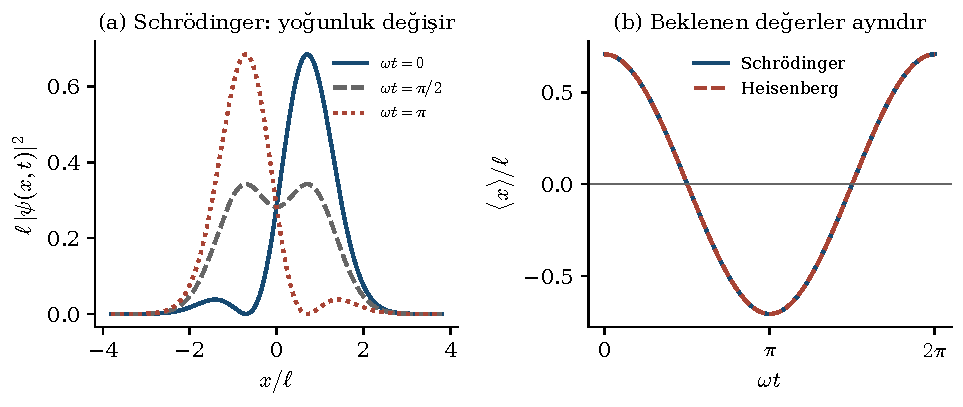
\includegraphics[width=\linewidth]{figurler/06_resimler.pdf}
 \caption[Schrödinger ve Heisenberg resimlerinin karşılaştırılması]{
 $(|0\rangle+|1\rangle)/\sqrt2$ başlangıç durumunda harmonik salınıcı.
 Solda Schrödinger resmindeki konum yoğunluğunun farklı zamanları,
 sağda ise iki resimden ayrı ayrı hesaplanan aynı
 $\langle x\rangle(t)$ eğrisi gösterilmiştir.
 $\ell=\sqrt{\hbar/(m\omega)}$'dır.}
 \label{fig:06_resimler}
\end{figure}

\BolumKaynakcaBitir
\end{document}
